\section{Introduction} 
\label{sec:intro}

% \jiahuan{@Minjia, need help to revise it, to remove the ``feedback''}
% \minjia{I rewrote the intro. Please take a look at blue text. If it looks good to you, remove the text color.}
% \jiahuan{I went through, fixed some inconsistency and shorten some sentences. I left some comments, please check it}

% Large Language Models (LLMs) have emerged as cornerstone of modern AI applications, serving billions of requests in applications ranging from chat assistants~\cite{chatgpt,gemini}, code generation tools~\cite{copilot,cursor}, and increasingly, real-time agentic systems~\cite{langchain,wu2024autogen}.
% Given LLMs are deployed in production at unprecedented scale, inference energy consumption significantly increases the total ownership of cost (TOC) and has become a major concern for sustainability~\cite{patel2024characterizing}. Recent studies show that LLM inference can account for over 90\% of AI infrastructure utilization for companies~\cite{desislavov2023trends}, significantly pressuring power delivery and thermal limits in data centers. For context, large datacenters are estimated to consume power for up to 2 million households~\cite{chien2023reducing,kemene2024ai}. 

% At the same time, LLM applications are increasingly latency-sensitive, especially in interactive and real-time settings. \textit{Service Level Objectives} (SLOs), such as \textit{Time-To-First-Token} (TTFT) and \textit{Inter-Token Latency} (ITL), are critical~\cite{agrawal2025evaluating, nie2024aladdin,shen2025accelgen}, and violating these SLOs degrades not only user experience but also downstream system responsiveness such as agentic pipelines~\cite{WebPilot}.
% For example, agent planning and dialog continuation are highly sensitive to ITLs which can lead to degraded performance for many applications~\cite{WebPilot, kang2025winfastloseslow, serverlessllm, zhao-etal-2024-enhancing-zero, wang2024revisitingslogoodputmetrics}.
% As LLMs are integrated into more interactive pipelines, SLO-aware serving is becoming very desirable. As such, it raises a key challenge: how can we serve LLMs under SLO constraints while reducing the system's energy footprint?

Large Language Models (LLMs) have become the cornerstone of modern AI services, powering applications ranging from conversational assistants~\cite{chatgpt,gemini}, code generation tools~\cite{copilot,cursor}, and agentic systems~\cite{zhang2025webpilot,wu2024autogen}.
Recent studies show that LLM inference now accounts for over 90\% of total AI infrastructure utilization for major providers~\cite{desislavov2023trends}.
As these systems are deployed at massive scale, inference energy consumption has emerged as one of the most critical bottlenecks to sustainable and cost-effective AI operation.
Recent industry reports indicate that even major cloud providers are constrained by power delivery limits, not just hardware availability~\cite{elsworth2025measuring,patel2024characterizing}.
% , e.g., Microsoft's CEO recently remarked that company does not have enough electricity to install all the AI GPUs in its inventory~\cite{}.
% ``you may actually have a bunch of chips sitting in inventory that I can’t plug in". 
% Industry-scale studies from Google, Microsoft, NVIDIA, OpenAI further confirm that LLM energy efficiency is now a first-order constraint for hyper-scale deployment~\cite{elsworth2025measuring,patel2024characterizing}.
This industry-wide inflection highlights a fundamental tension between performance scaling and energy capacity: data centers can no longer rely on simply provisioning more accelerators to sustain model growth, which motivates energy-efficient LLM serving as a primary design goal.
% Recent studies show that LLM inference can account for over 90\% of AI infrastructure utilization for companies~\cite{desislavov2023trends}, significantly pressuring power delivery and thermal limits in data centers. For context, large datacenters are estimated to consume power for up to 2 million households~\cite{chien2023reducing,kemene2024ai}. 



While the conventional wisdom of dynamic frequency scaling-based energy control holds that reducing frequency directly lowers power~\cite{gonzalez1997supply}, the net effect on energy (time $\times$ power) for LLM serving is not straightforward, as the increase in latency, which is crucial for user experience, varies significantly depending on workload characteristics.
In particular, our empirical profiling of LLM inference
reveals an interesting non-monotonic energy-frequency relationship.
As shown in \fref{fig:u-shape-coupled}, while reducing A100 GPU frequency from 1410 MHz to 1005 MHz ($-28.7\%$) does increase execution time, this increase is sub-linear.
Consequently, the total energy follows a U-shaped curve with respect to frequency.
This U-shaped trend suggests that at low frequencies, execution time dominates energy, whereas at high frequencies, power dominates; in the middle lies an energy sweet spot.

\begin{figure}[!t]
    \centering
    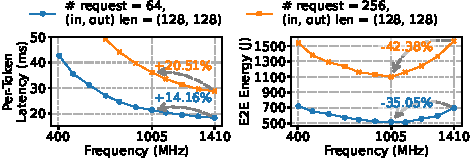
\includegraphics[width=\columnwidth]{figs/u-shaped-intro.pdf}
    \caption{The decreasing per-token latency and the U-shaped energy-frequency curve across varying GPU frequencies, for LLaMA-3.1-8B~\cite{grattafiori2024llama} served on an A100 with SGLang~\cite{zheng2024sglang}.}
    \label{fig:u-shape-coupled}
\end{figure}

% While this observation indicates a clear optimization opportunity, its practical realization for LLM inference faces several challenges.
% First, 
% % due to the increased latencies under lower frequency, 
% many systems leverage token-level batching to amortize overheads and improve GPU utilization. However, batching prefill and decode tokens together makes it difficult to control energy without compromising phase-specific SLO targets (\sref{sec:obs-u-shape}). 
% Second, real-world workloads exhibit strong temporal variations in both arrival rates and request types, which lead to shifting prefill-decode throughput demand, calling for highly adaptive control policies (\sref{subsec:temporal-variation}).
% Third, energy efficiency also depends on low-level execution.
% We find that batch size boundaries introduce subtle implication to LLM decode execution. When batch sizes cross specific thresholds (e.g., 128), GPU becomes underutilized, creating ``staircases'' in \textit{Energy-Per-Output-Token} (\fref{fig:kernel-tile}).
% This interaction between execution and energy usage is not well-studied in existing literature (\sref{subsec:tile-effect}).

% \jiahuan{We should rearrange this paragraph to make it consistent with observation section. I write the new version of this paragraph. My idea is \begin{enumerate}
%     \item cannot directly apply traditional DVFS due to latency SLOs.
%     \item P/D contention in coupled architecture (\appref{subsubsec:pd-interference})
%     \item there are 3 challenges \begin{enumerate}
%         \item Real-world workloads exhibit strong temporal variations in two time scales, long-term P/D demand shifting and short-term workload fluctuation (\sref{subsec:temporal-variation})
%         \item the phase-specific U-shaped relationship \sref{sec:obs-u-shape}
%         \item the architectural-induced inefficiency ((\sref{subsec:tile-effect}))
%     \end{enumerate}
%     \item then in the next paragraph, we can introduce the P/D disaggregated naturally. Old version is jumpy
% \end{enumerate}}
% \minjia{Looks good. Avoid referencing appendix in the intro. Immediately viewed as not self-contained.}

While this observation exposes a promising optimization opportunity, unfortunately what works well for conventional data center frequency control does not directly translate to energy-efficient LLM serving.
LLM applications are often real-time and interactive, with phase-specific \textit{Service Level Objectives} (SLOs), including \textit{Time-To-First-Token} (TTFT) and \textit{Inter-Token Latency} (ITL).
Violating these SLOs degrades user experience and downstream system responsiveness such as agentic pipelines~\cite{zhang2025webpilot}.
Modern LLM serving systems commonly employ continuous batching~\cite{yu2022orca} to batch prefill and decode tokens together for higher GPU utilization.
However, this coupled design introduces latency contention and phase interference~\cite{zhong2024distserve}, making it difficult to control energy without violating distinct, phase-specific SLOs.
Furthermore, achieving energy savings without SLO violations is complicated, and our analysis reveals several insights:
\emph{Insight-1}: Real-world workloads exhibit strong temporal variations in request rates and types, which lead to shifting prefill-decode throughput demand and short-term workload fluctuations.
For effectiveness, an energy controller must be adaptive and responsive (e.g., able to react on timescales of tens of milliseconds), but most static and power-capping methods incur coarse, high-latency adjustments (\sref{subsec:temporal-variation}).
\emph{Insight-2}: The energy-latency trade-off is neither uniform nor monolithic.
The prefill and decode phases have different U-shaped energy-frequency relationships and latency-frequency sensitivities.
This implies that a single, coupled frequency policy is inherently suboptimal and makes it difficult to meet distinct, phase‑specific SLOs (\sref{sec:obs-u-shape}).
\emph{Insight-3}: Energy efficiency also depends on architectural execution granularity.
We observe that when decode batch sizes cross certain thresholds (e.g., 256), GPU kernel tiling shift discontinuously, leaving compute units idle and creating a ``staircase'' pattern in latency and energy curves (\sref{subsec:tile-effect}).

% \old{
% While this observation exposes a promising optimization opportunity, unfortunately what works well for conventional data center frequency control does not directly translate to energy-efficient LLM serving for several reasons.
% LLM applications are often deployed in interactive and real-time settings, with phase-specific \textit{Service Level Objectives} (SLOs), such as \textit{Time-To-First-Token} (TTFT) and \textit{Inter-Token Latency} (ITL).
% Violating these SLOs degrades not only user experience but also downstream system responsiveness such as agentic pipelines~\cite{WebPilot}.
% Achieving energy saving without SLO violations is complicated by several challenges:
% \emph{Insight-1}:
% Real-world workloads exhibit strong temporal variations in arrival rates and request types, which lead to shifting prefill-decode throughput demand and short-term workload fluctuations, calling for highly adaptive control policies (\sref{subsec:temporal-variation}).
% To remain effective, an energy controller must be responsive, e.g., able to react on tens of millisecond timescales, but most DVFS and power-capping methods incur coarse, high-latency adjustments.
% \emph{Insight-2}:
% Modern LLM serving systems often use continuous batching~\cite{orca} to combine prefill and decode tokens together to improve GPU utilization.
% This coupled design makes it difficult to control energy without violating distinct, phase-specific SLO targets (\sref{sec:obs-u-shape}).
% \jiahuan{it seems in insight we talk about the U-shaped figure, not P/D interference}
% \emph{Insight-3}:
% Energy efficiency also depends on architectural execution granularity.
% We observe that when decode batch sizes cross certain thresholds (e.g., 256), GPU kernel tiling shift discontinuously, leading compute units idle and creating ``staircases'' pattern in \textit{Energy-Per-Output-Token} (EPOT) (\sref{subsec:tile-effect}).
% }

% \jiahuan{Furthermore, modern LLM serving systems often use continuous batching~\cite{orca} to combine prefill and decode tokens together to improve GPU utilization.
% This coupled design makes it difficult to control energy without violating distinct, phase-specific SLO targets. (can mention \appref{subsubsec:pd-interference})}

% \jiahuan{after reviewing the background section, I believe the current writing is enough to explain the interference of co-located architecture, if the reviewers have background. I will add a small section in \appref{subsubsec:pd-interference} to provide more details about that, in case that some reviewers may not fully get it.}

% \minjia{I revised the text to make the lightweight and responsive frequency control challenge stand out earlier. However, how are we going to convince people this is an important challenge to solve, e.g., why simply placing a power cap during night time or some coarse-grained DVFS methods won't work?}
% \jiahuan{simple power cap during night time is not adaptive enough, i.e., there are also low-load time during the day, and request brustiness at night.}
% \jiahuan{in \fref{fig:time-window} I show the coarse-grained frequency control harm the TTFT SLO attainment, as the prefill instance is largely stateless, request length can change rapidly between consecutive iteration. Should we mention it in the observation section?}
% \minjia{Right. We need some motivating example for having lightweight and responsive frequency control. Otherwise, people will miss this design. Having some results to show that coarse-grained control easily hurts SLO attainment and add that in the observation (perhaps when talking about temporal variation) would be good. It also makes the Insight 2's claim that "one-size-fit"all" stronger (not only OFA does not work but also coarse-grained control also is also sub-optimal).}
% \jiahuan{my idea is, \sref{subsec:temporal-variation} seems a little redundant, we can justify the choice of P.D disaggregation architecture in other ways, and mention the necessity of iteration-level responsiveness}
% \minjia{Maybe, but if you agree with the above comment, then let's add the results that coarse-grained frequency control is sub-optimal? }
% \jiahuan{you mean add it to observation section or analysis result section? Currently \fref{fig:time-window} is in the analysis result section. If we want to explain the necessity of per-iteration frequency control, we can simply move \fref{fig:prefill-tokens-fluctuation} to the observation section. It shows the quick workload changes in prefill instance.}
% \minjia{I mean adding the results to the observation section to motivate the necessity of having fine-grained frequency control.}


% To address these challenges, we turn to a new architectural trend in LLM serving systems: prefill-decode (P/D) disaggregation~\cite{patel2024splitwiseefficientgenerativellm,zhong2024distserve} and present \name, a novel system for SLO-aware and energy-optimized LLM inference.

% \jiahuan{I moved original Insight-2 here.}

To address these challenges, we build upon prefill-decode (P/D) disaggregation~\cite{patel2024splitwise,zhong2024distserve} and present \name, 
the first energy-efficient SLO-aware disaggregated LLM serving system that jointly optimizes GPU frequency and request routing under latency SLOs.
Specifically, \name introduces three key techniques:
(1) \governor (\sref{subsec:governor}), a responsive frequency controller that adjusts GPU frequency at fine-grained, \cameraready{per-iteration granularity within inference engine} to respond to instantaneous workload fluctuations while adhering to SLOs;
(2) \predictor (\sref{subsec:predictor}), a lightweight yet accurate model inference time predictor, trained offline from profiling data and continuously adapted online to maintain accuracy under dynamic workloads and frequencies;
(3) \router (\sref{subsec:router}), an architecture-aware, state-space guided request router that dynamically steers decode requests by navigating a load-frequency state space to maximize overall energy efficiency while meeting SLOs.
Together, these techniques allow \name to jointly optimize for SLO attainment, energy efficiency, and dynamic load adaptation.

We implement \name on SGLang~\cite{zheng2024sglang}, a production-grade LLM inference engine, and make the following contributions:
\textbf{(1)} We propose the first optimization framework for energy efficient LLM inference under P/D disaggregation, which enables principled control of energy-latency trade-offs under SLO constraints.
\textbf{(2)} We are the first to identify two new architectural phenomena in disaggregated LLM serving: phase-specific U-shaped energy-frequency relationships and architectural granularity-induced inefficiency, which motivate phase-specific and architecture-aware energy control.
\textbf{(3)} We design and implement \name, the first SLO-aware and energy-efficient disaggregated LLM serving system that incorporates phase-specific and responsive frequency controller, as well as state-space guided request routing that delivers the best energy-latency efficiency.
We conduct extensive evaluations across various LLMs and workloads.
Our results show that \name achieves up to 36.3\% energy savings while preserving TTFT and ITL SLO attainment rates.




% \begin{itemize}
%     \item To the best of our knowledge, we present the first formal formulation of energy efficiency optimization for LLM inference under a P/D disaggregated architecture, while highlighting its connection to control theory and phase-specific scheduling.
%     \item We design and implement \name, an SLO-aware and energy-efficient LLM serving system that incorporates phase-specific feedback-driven frequency control, state space navigation-based router, and lightweight yet accurate latency prediction model. 
%     \item We conduct extensive evaluations across state-of-the-art LLMs and various workloads. Our results show that \name achieves up to 36.3\% energy savings while preserving SLO attainment rates. 
% \end{itemize}



